\documentclass[UTF8]{ctexart}
\usepackage[a4paper, top=25.4mm, bottom=25.4mm, left=31.8mm, right=31.8mm]{geometry}
\usepackage{graphicx}
\usepackage{amsmath}
\usepackage{multirow}
\usepackage{subcaption}
\usepackage{tabu}
\usepackage{minted}
\usemintedstyle{manni}
\usepackage[table]{xcolor}

\setlength{\parskip}{1em}
\definecolor{lightergray}{gray}{0.95}

\begin{document}
\begin{titlepage}
  \begin{center}
    \vspace*{1cm}

    \Large
    编译原理

    \vspace{0.5cm}
    \Huge
    \textbf{词法分析实验实验报告}

    \vfill

    \normalsize\kaishu
    班级:07111603 \\
    学号:1120161730 \\
    姓名:武上博 \\
    \today
    \vspace{1cm}
  \end{center}
\end{titlepage}

\tableofcontents
\newpage

\section{实验目的}
\begin{enumerate}
  \item 熟悉 C 语言的词法规则,了解编译器词法分析器的主要功能
  \item 掌握典型词法分析器构造的相关技术和方法,设计并实现 C 语言词法分析器
  \item 掌握编译器从前端到后端各个模块的工作原理,词法分析模块与其他模块之间的交互过程
\end{enumerate}

\section{实验内容}
根据 C 语言的词法规则,设计并识别 C 语言所有单词类的词法分析器的确定有限状态自动机,并使用 Java、C/C++、Python 其中的任意一种语言,采用程序中心法或者数据中心法设计并实现词法分析器。词法分析器的输入为 C 语言源程序,输出为属性字流。

\section{实验的具体过程步骤}
\subsection{程序实现的大致思路}
为了和接下来语法分析模块相配合,本次实现的词法分析器接受 C 语言源程序作为输入,利用 XML 作为格式进行输出分析的词法内容。同时,为了和 BIT-MiniCC 进行更好的整合,本次实验我决定使用 Python 作为主语言进行各个模块的实现。

经过分析,我觉得本次实验中词法分析器是如下的大致构造:

\begin{figure}[h]
  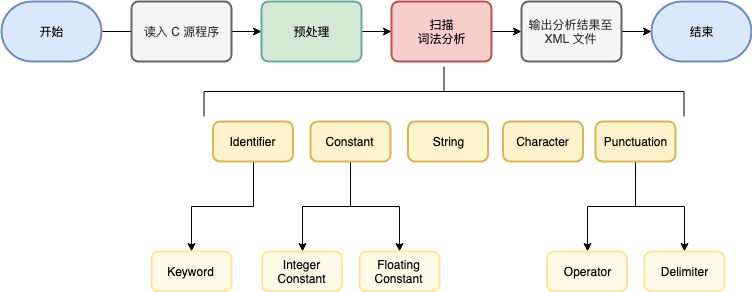
\includegraphics[width=\linewidth]{images/lexical.png}
  \caption{词法分析器的大致流程}
  \label{fig:figure1}
\end{figure}

也就是说,我们本次需要实现的模块有:

\begin{enumerate}
  \item 文件读入
  \item 程序预处理模块(去除每行前部分空格、注释等)
  \item 进行词法分析,依次识别:
  \begin{itemize}
    \item 标识符 Identifier
    \item 常量 Constant
    \begin{itemize}
        \item 整数型常量 Integer Constant
        \item 点型常量 Floating Constant
    \end{itemize}
    \item 字符 Char
    \item 字符串 String
    \item 算符 Punctuation
      \begin{itemize}
        \item 运算符 Operator
        \item 界限符 Delimiter
      \end{itemize}
  \end{itemize}
  \item 输出 XML 文件
\end{enumerate}

\subsection{具体模块的实现}

接下来,我们分别对各个模块相应的具体实现方法进行介绍。

\subsubsection{程序输入和预处理}

本次实验中的输入是一个 C 语言程序的源文件。我们从命令行读入需要处理的文件路径,处理文件内容。

\begin{minted}
[
  linenos,
  frame=lines,
  framesep=2mm
]
{python}
def main():
  # Print usage if arguments are not legal
  if len(sys.argv) < 2:
    print('[Usage] ./scan.py <C source file path>')
    sys.exit(0)

  # Read file from file path taken from command line arguments
  filePath = sys.argv[1]
  with open(filePath, 'r', encoding='utf-8') as f:
    content = f.readlines()

\end{minted}

在读文件时,我使用了 \texttt{readlines()} 函数为了逐行读入文件。我们得到 \texttt{content},也就是代码的基本内容。之后,我们对读入的内容进行预处理。

\begin{minted}[
  linenos,
  frame=lines,
  framesep=2mm
]{python}
# 主函数内的内容
# Pre process C source file
code = preProcess(content)
# 预处理函数
def preProcess(content):
  code = ''
  # Trim leading white space 去掉每行最前面的空白
  for line in content:
    if line != '\n':
      code = code + line.lstrip()
    else:
      code = code + line
  return code
\end{minted}

我首先定义代码变量 \texttt{code},之后按行处理代码内容,对于每一行代码,如果代码不是空行,那么我就将这一行的代码和前面定义的 \texttt{code} 相连接,之后我们只需要处理 \texttt{code} 缓冲区内的代码内容即可。

\subsubsection{标识符 Identifier 的判断}

\subsubsection{常量(整形常量 Integer Constant 和浮点型常量 Floating Constant)的判断}

\subsubsection{字符 Character、字符串 String 的判断}

\subsubsection{算符(包括运算符 Operator 和界限符 Delimiter)的判断}

\section{实验结果}

\section{实验心得体会}
\end{document}